\documentclass{beamer}

\usepackage{movie15}
\usetheme{Marburg}
\usecolortheme{lily}

\title{Demystifying the Domain Registration}
\author{Katie Ford}
\date{\today}

\begin{document}

\frame{\titlepage}

% INTRODUCTION
\section[Outline]{}
\frame{\tableofcontents}
\frame{
	\frametitle{Me}
	\begin{columns}
	\begin{column}{0.5\textwidth}
		\begin{center}
		
\includegraphics[width=4cm]{katie.jpg}
		\end{center}
	\end{column}
	\begin{column}{0.6\textwidth}
		\begin{center}
		Katie Ford\\
		Domains Team\\
		\\
		\includegraphics[width=0.5\textwidth]{dh.png}
		\end{center}
	\end{column}
	\end{columns}
}

% PLAYERS
\section{Players}
\frame{
	\frametitle{Players}
	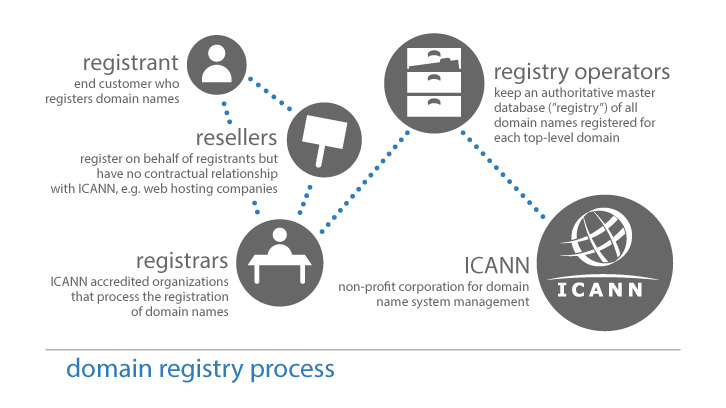
\includegraphics[width=\textwidth]{regprocess.png}
}

\frame{
	\frametitle{ICANN}
	\begin{center}
	aka\\
	Internet Corporation for Assigned Names and Numbers
	\end{center}
	\pause
	
\includegraphics[width=\textwidth]{icant.jpg}
}

\frame{
	\frametitle{ICANN}
	\begin{itemize}
		\item Approves price changes
		\item Creates some policies (e.g. IRTP lock)
		\item Accredit Registrars and Registries
	\end{itemize}
}

\frame{
	\frametitle{Registry/Provider}
	\begin{itemize}
		\item Sets base price
		\item Creates most policies
		\item Examples:
			\begin{itemize}
			\item Verisign
			\item PIR
			\item Donuts
			\item Nominet
			\end{itemize}
	\end{itemize}
}

\frame{
	\frametitle{Registrar}
	\begin{itemize}
		\item Maintains WHOIS server
		\item Email expiration reminders
	\end{itemize}
}

\frame{
	\frametitle{Registrant}
	\pause
	
\includegraphics[width=\textwidth]{me.jpg}
}

% TLDs
\section{TLDs and Registries}

\frame{
	\frametitle{TLDs and Registries}
}

\frame{
	\frametitle{ccTLDs}
	\begin{itemize}
	\item 2-letter tlds
	\item Each country (plus some bonuses) have one
	\item Not subject to ICANN
	\item Examples:
		\begin{itemize}
		\item .us
		\item .uk, .co.uk, .org.uk
		\item .io
		\item .tv
		\end{itemize}
	\end{itemize}
}

\frame{
	\frametitle{gTLDs}
	\begin{itemize}
		\item Subject to ICANN
		\item Examples
			\begin{itemize}
			\item blog
			\item dog
			\item recipes
			\item shop
			\end{itemize}
	\end{itemize}
}

% Things to look out for
\section{Things to look out for}
\subsection{Premium}
\frame{
	\frametitle{What does "premium" mean?}
	\pause
	
\includegraphics[width=\textwidth]{jetsonmoney.jpg}
}

\frame{
	\begin{figure}
		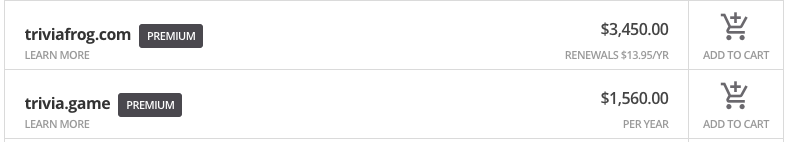
\includegraphics[width=\linewidth]{premiumss.png}
		\caption{Screen shot of premium domains for sale}
	\end{figure}
}

\frame{
	\frametitle{Registry-designated}
	\begin{itemize}
		\item{Price determined in part by the registry}
		\item{Higher renewal costs}
		\item{Limited Registrars and Resellers}
	\end{itemize}
}


\frame{
	\frametitle{Secondary-market domains}
	\begin{itemize}
		\item{Sold by 3rd parties}
		\item{Regular domains}
	\end{itemize}
}

\subsection{Other}

\frame{
	\frametitle{Things to look out for in Registrars}
	\begin{itemize}
		\item brokerage services
		\item premium domains
	\end{itemize}
}

\frame{
	\frametitle{Extended Attributes}
	\includegraphics[width=\linewidth]{caattribute.png}
	Extended attribute for .ca
}

\frame{
	\frametitle{Registry Policies}
	\begin{itemize}
		\item no transfer
		\item autorenew only
		\item theft protection
		\item has premium domains
	\end{itemize}
}

\frame{
	\frametitle{The End}
	\begin{center}{https://github.com/ClassicKatie/wcbham17}\end{center}
	
\includegraphics[width=\textwidth]{theend.jpg}
}


\end{document}